\makeatletter
\def\@makechapterhead#1{%
  \vspace*{10\p@}%
  {\parindent \z@ \raggedleft \normalfont
    \ifnum \c@secnumdepth >\m@ne
      \if@mainmatter
        \LARGE\bfseries \@chapapp\space \thechapter
	\vskip 4pt
        \hrule height 2pt
        \par\nobreak
        \vskip 5\p@
      \fi
    \fi
    \interlinepenalty\@M
    \huge \bfseries #1\par\nobreak
\vskip 5pt

\hrule height 2pt   
 \vskip 10\p@  
  }}
\makeatother

\chapter{Flip Flops}\label{chap6}
\addtocontents{toc}{\protect\contentsline{chapter}{\protect Chapter \numberline{\thechapter.}
Flip Flops}{\thepage--\pageref{6end}}}  

\section{Introduction}\label{sec6.1}
The logic circuits whose outputs at any instant of time depend only on
the input signals present at that time are known as combinational
circuits. But the logic circuits whose outputs at any instant of time
depend not only on the present inputs but also on the past outputs are
called requential cirduits. In sequential circuits, the output signals
are feed back to the input side. Thus, an output signals are a function
of the present input signals and the past output signals. The block
diagram of a sequential circuit is shown in Fig.~\ref{fig6.1}  below.
\begin{figure}[H]
\centering
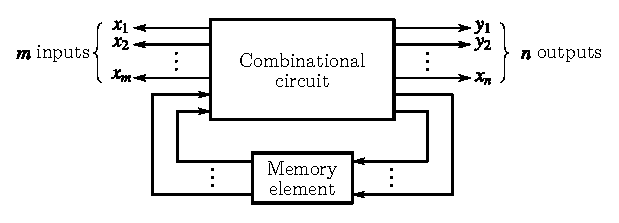
\includegraphics[scale=1.1]{chap6/fig6.1.eps}
\caption{Block diagram of a sequential circuit}\label{fig6.1}
\end{figure}

It consists of a combinational circuit to which memory elements are
added to form a feedback path. The memory elements are devices capable
of storing binary information within them. The memory elements which
are used in requential circuit are called flip-flops. A flip-flop is
also called as latch. Each flip-flop is capable of storing one bit of
information and has 2 outputs Q \& $\overline{\rmQ}$ which are complement
to each other.

\section{NAND gate latch}\label{sec6.2}
A NAND gate latch is obtained by connecting two NAND gates back to
back as shown in Fig.~\ref{fig6.2}(a) below. Its logic symbol and
truth table is given in Fig.~\ref{fig6.2}(b) \& (c) respectively.
\begin{figure}[H]
\centering
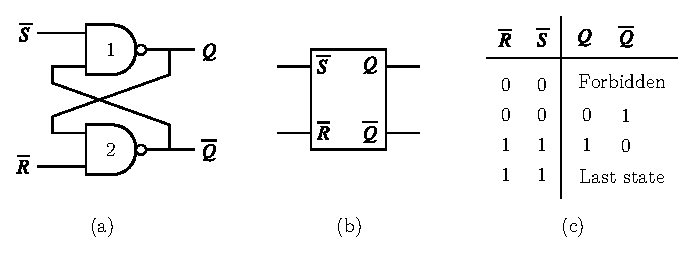
\includegraphics[scale=1.05]{chap6/fig6.2.eps}
\caption{NAND gate latch}\label{fig6.2}
\end{figure}

\heading{When {\boldmath{$\overline{\rmR}=0 ~\&~ \overline{\rmb} = 0$}}} : When
an input to a NAND gate is `0', the output is 1. $\therefore ~ \overline{\rmR}
= 0 ~\&~ \overline{\rmS} = 0$ would try to make both Q and $\overline{\rmQ}$ equal
to 1 (i.e., $\rmQ=\overline{\rmQ} =1$) which is not possible. So $\overline{\rmR} =
0$ \& $\overline{\rmS}=0$ is forbidden.

\heading{When {\boldmath{$\overline{\rmR}=0 ~\&~ \overline{\rmS} = 1$}}} : When
$\overline{\rmR} =0$ then $\overline{\rmQ} =1$ which results in $\rmQ=0$. Thus $\rmQ=0$ and
$\overline{\rmQ} =1$.

\heading{When {\boldmath{$\overline{\rmR}=1 ~\&~ \overline{\rmS}=0$}}} : When
$\overline{\rmS}=0$ then $\rmQ = 1$ which results in $\overline{\rmQ} =0$. Thus $\rmQ=1$
and $\overline{\rmQ}=0$.

\heading{When {\boldmath{$\overline{\rmR}=1 ~\&~ \overline{\rmS}=1$}}} : Initially
assume that $\rmQ=1 (\overline{\rmQ}=0)$. Then the inputs to gets 1 are
$\overline{\rmS}=1$ and $\overline{\rmQ}=0$, ~~$\therefore ~$ $\rmQ =1$, then the inputs to
gate 2 are $\overline{\rmR}=1$ and $\rmQ =1$, ~~$\therefore$ $\overline{\rmQ} =0$. So there
is no change in the state.

\begin{problem}\label{prob6.1}
If the waveform in Fig.~P6.1 below are applied to an NAND gate
latch (shown in Fig.~\ref{fig6.2}), sketch the resulting output
waveforms Q and $\overline{\rmQ}$ related to the inputs. Assume the Q
starts low.
\begin{figure}[H]
\centering
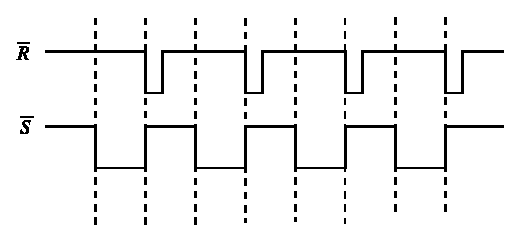
\includegraphics[scale=1.05]{chap6/sol.6.2.1(a).eps}

\medskip
{\bf Fig.~P6.1}
\end{figure}
\end{problem}

\eject

\begin{solution}
~
\begin{figure}[H]
\centering
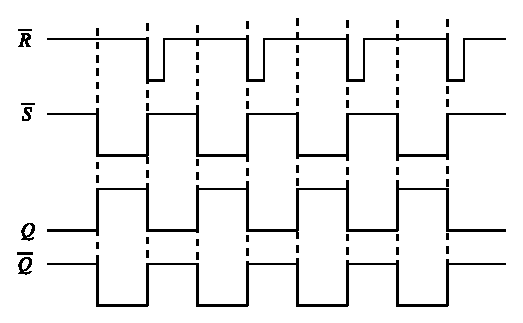
\includegraphics[scale=1.05]{chap6/sol6.2.1.eps}


\medskip
{\bf Fig.~S6.1}
\end{figure}
\end{solution}

\section{NOR gate latch}\label{sec6.3}
A NOR gate latch is obtained by connecting two NOR gates back to back
as shown in Fig.~\ref{fig6.3}(a) below. The logic symbol and truth
stable is given in Fig.~\ref{fig6.3}(b) \& (c) respectively.
\begin{figure}[H]
\centering
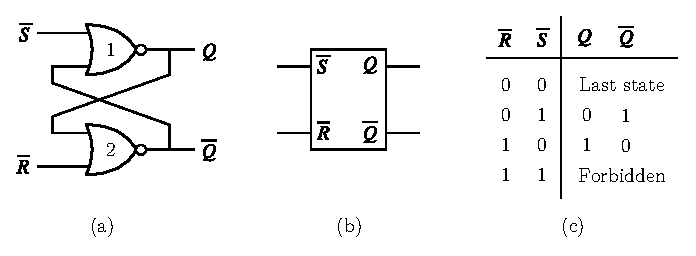
\includegraphics[scale=1.05]{chap6/fig6.3.eps}
\caption{NOR gate latch}\label{fig6.3}
\end{figure}

\heading{When \boldmath{$\overline{\rmR}=0 ~\&~ \overline{\rmS} =0$}} :~ Initially assume
that $\rmQ =1 (\overline{\rmQ}=0)$. Then the inputs to gate 1 are
$\overline{\rmS}=0$ and $\overline{\rmQ}=0$. ~~$\therefore$ ~~$\rmQ = 1$, then the inputs
to gate 2 are $\overline{\rmR}=0$ and $\rmQ=1$. ~~$\therefore~~ \overline{\rmQ}=0$. So there in no change in the state.

\heading{When \boldmath{$\overline{\rmR} =0 ~\&~ \overline{\rmS}=1$}} :~ When $\overline{\rmS}=1$
then $\rmQ =0$ which results in $\overline{\rmQ} =1$.

\eject

\heading{When \boldmath{$\overline{\rmR} =1 ~\&~ \overline{\rmS} =0$}} :~ When $\overline{\rmR} =1$ then
$\overline{\rmQ} =0$ which results in $\rmQ =1$.


\heading{When \boldmath{$\overline{\rmR}=1 ~\&~ \overline{\rmS} =1$}} :~ When an input to a NOR
gate is 1, the output is 0. $\therefore$~ $\overline{\rmR} = 1 ~\&~ \overline{\rmS}
=1$ would try to make both Q and $\overline{\rmQ}$ equal to 0 (i.e., $\rmQ
= \overline{\rmQ}=0$) which is not possible. So $\overline{\rmR} =1 ~\&~ \overline{\rmS} =1$
is forbidden.

\section{RS Flip Flop}\label{sec6.4}

A RS Flip-flop has 2 inputs R(RESET) and S(SET) and two outputs Q and
$\overline{\rmQ}$. As mentioned, the two outputs ($\rmQ~\&~\overline{\rmQ}$) are
complement to each other. A RS flip-flop is set ($\rmQ=1$ \&
$\overline{\rmQ}=0$) when $\rmS=1$ and $\rmR=0$ and it is reset
($\rmR=0 \& \overline{\rmQ}=1$) when $S=0$ and $R=1$. A RS flip-flop can be
constructed using NAND or NOR gates in different
ways. Fig.~\ref{fig6.4}(a) shows one possible RS flip-flop using NAND
gates only and Fig.~\ref{fig6.4}(b) \& (c) shown its logic symbol and
truth table respectively.
\begin{figure}[H]
\centering
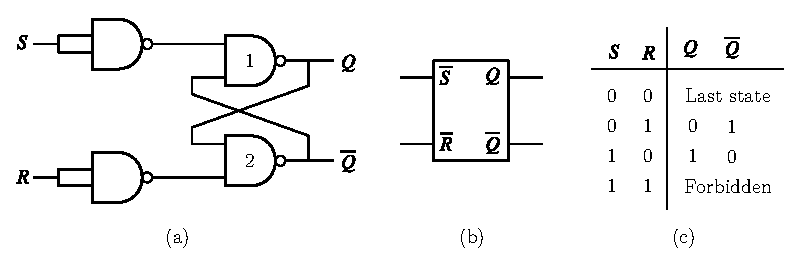
\includegraphics{chap6/fig6.4.eps}
\caption{RS flip flop}\label{fig6.4}
\end{figure}

\begin{problem}\label{prob6.2}
Find the output Q and $\overline{\rmQ}$ for S and R waveform shown below in
Fig. P6.2 below. Initially assume $\rmQ =0$.
\begin{figure}[H]
\centering
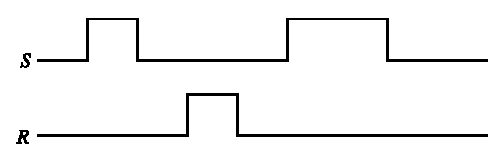
\includegraphics{chap6/fig.6.4.1(a).eps}

\medskip
{\bf Fig.~P6.2}
\end{figure}
\end{problem}

\eject

\begin{solution}
~
\begin{figure}[H]
\centering
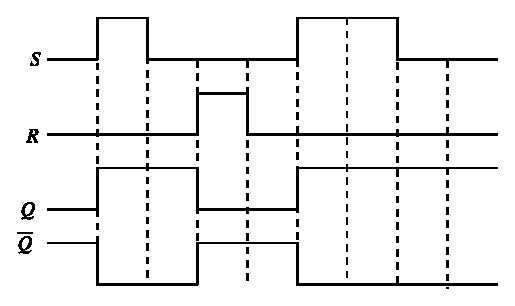
\includegraphics{chap6/sol6.4.1.eps}

\medskip
{\bf Fig.~S6.2}
\end{figure}
\end{solution}

\section{Clocked RS Flip Flop}\label{sec6.5}
A clocked RS flip-flop is shown in Fig.~\ref{fig6.5} below.
\begin{figure}[H]
\centering
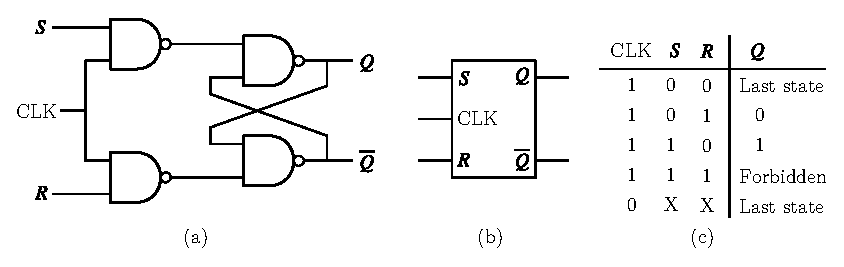
\includegraphics{chap6/fig6.5.eps}
\caption{}\label{fig6.5}
\end{figure}


When the clock CLK is HIGH, the output of the 2 input NAND gates are
$\overline{S}$ and $\overline{R}$. Thus the latch operates normally. When the
clock CLK is LOW, the output of the 2 input NAND gates are 1 which
results is forbidden.

\eject

\begin{problem}\label{prob6.3}
For a clocked R-S latch, determine the Q and Q outputs for the given
input Fig.~P6.3.
\begin{figure}[H]
\centering
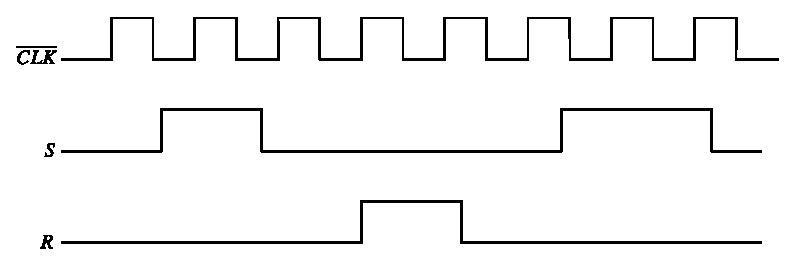
\includegraphics{chap6/figP6.5.eps}

\medskip
{\bf Fig.~P6.3}
\end{figure}
\end{problem}

\begin{solution}
~
\begin{figure}[H]
\centering
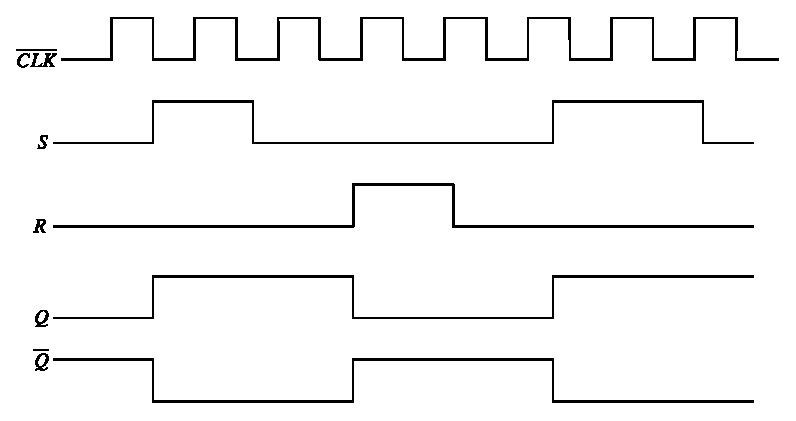
\includegraphics{chap6/figA6.5.eps}

\medskip
{\bf Fig.~S6.3}
\end{figure}
\end{solution}

\label{6end}
